\documentclass{article}
\usepackage{graphicx}
\usepackage{listings}
\usepackage[strings]{underscore}

\begin{document}
\section{To get to know the GPU:}
\begin{lstlisting}[language=Python]
from numba import cuda
cuda.detect()
\end{lstlisting}
\begin{verbatim}
-> Results:
Found 1 CUDA devices
id 0                Tesla T4                              [SUPPORTED]
                      Compute Capability: 7.5
                           PCI Device ID: 4
                              PCI Bus ID: 0
                                    UUID: GPU-0c40aef4-a85b-6723-4274-1db8dde9d5a1
                                Watchdog: Disabled
             FP32/FP64 Performance Ratio: 32
Summary:
	1/1 devices are supported
\end{verbatim}

\section{To choose the GPU device}
\begin{lstlisting}[language=Python]
cuda.select_device(0)
\end{lstlisting}
\begin{verbatim}
-> Results:
<weakproxy at 0x7ad02976f290; to 'numba.cuda.cudadrv.driver.Device' at 0x7ad017b963c0>
\end{verbatim}

\section{Proof}

\begin{figure}[htbp]
    \centering
    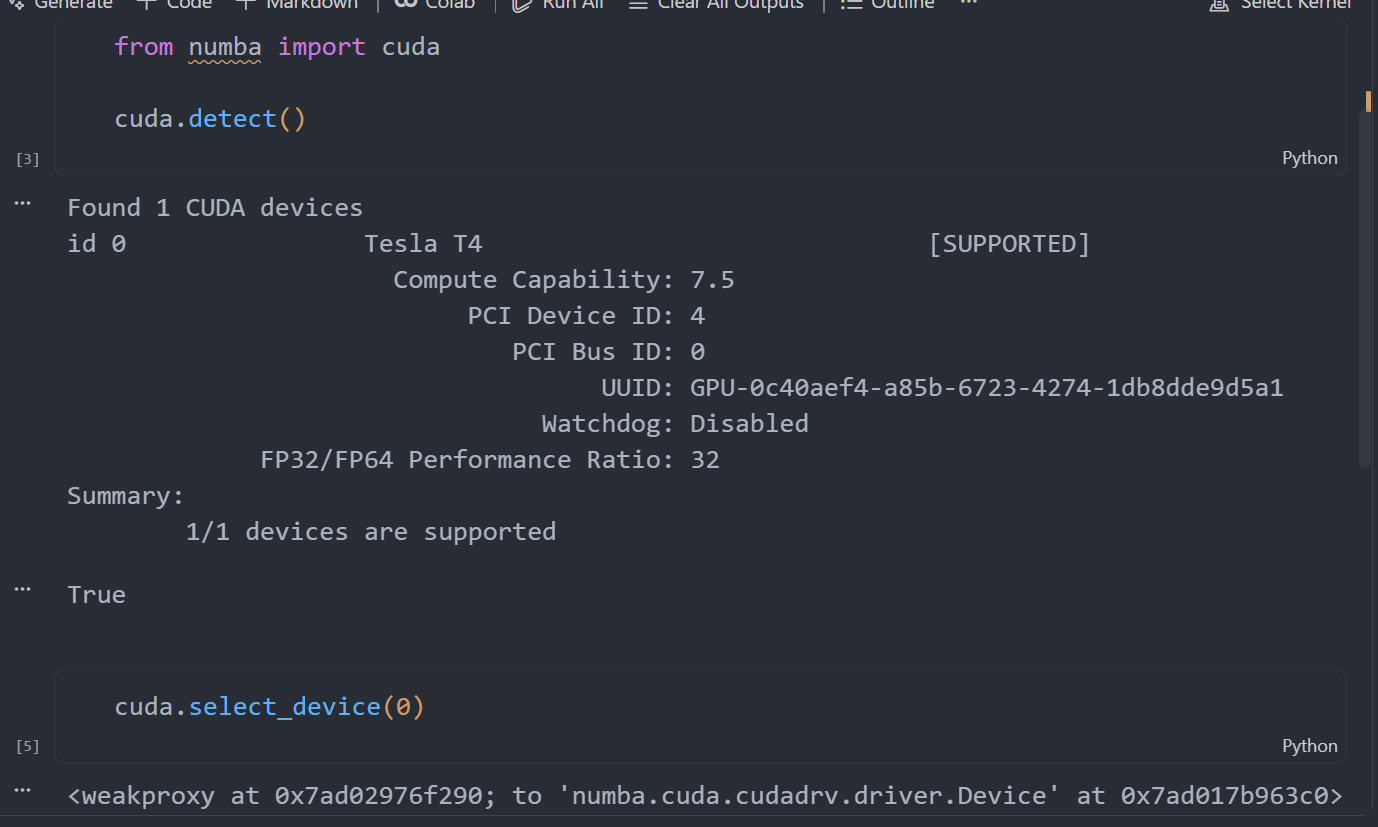
\includegraphics[width=0.85\textwidth]{Result.png}
    \caption{GPU detection result}
\end{figure}
\end{document}
